\newpage\section{Design and Development of the Artefacts}

The artifact, which is intended to improve experimental research in behavioral data analytics, is to be implemented as a software component or application. In this step, a suitable architecture is developed based on the established requirements. For this purpose, the basic technical framework and system architecture are presented first. Subsequently, the artifact is concretely conceptualized by elaborating different process steps of the application. Then, customizing and output capabilities of the final application are conceptualized and finally the user interface and specific components of the application.

\subsection{Technological Framework and System Architecture}

This section is intended to provide an overview of the technological framework used and the basic architecture of the application. This section focuses primarily on a basic overview, while the next sections go into more detail about the individual components.

\subsubsection{Java}

Java is a programming language originally developed by Microsystems. Since 2009 Java is part of the product portfolio of Oracle Corporation. Java is an object-oriented programming language, which makes it an universally applicable and robust programming language (\cite{Ullenboom.2017}).

Unlike many other programming languages, one of the special features of Java is its platform independence. Most programming languages use a compiler or interpreter to translate program code into byte code, which varies depending on the hardware and can only be executed on the appropriate processors. Java avoids this limitation by first having a compiler translate the Java program code into byte code, which is then executed in a virtual environment, the \ac{jvm}, with the help of an interpreter. In this way, Java code can theoretically be executed on any system (\cite{Ullenboom.2017}).

Java is not only a programming language, but also a runtime system, which Oracle wants to make clear with the term Java Platform. Thus, in addition to the Java programming language, there are certainly other languages that run a Java runtime environment, such as various scripting languages like Groovy (http://groovy-lang.org), JRuby (http://jruby.org), Jython (http://www.jython.org), Kotlin (http://kotlinlang.org) or Scala (http://www.scala-lang.org). Scripting languages on the Java platform are becoming more popular; they establish a different syntax but use the \ac{jvm} and libraries (\cite{Ullenboom.2017}).

Along with the programming language and \ac{jvm} comes a set of standard libraries for data structures, string processing, date/time processing, graphical interfaces, input/output, network operations, and more. This forms the basis for higher-level services such as database connections or web services. An integral part of the standard library since Java 1.0 are still threads. They are easy-to-create execution threads that can work independently of each other. In the meantime all popular operating systems support these \enquote{lightweight processes} by house, so that the \ac{jvm} does not have to reproduce these parallel program parts, but can refer to the operating system. On the new multi-core processors, the operating system ensures optimum utilization of the computing power, since threads can really work concurrently (\cite{Ullenboom.2017}).





Java ist eine Insel (\cite{Ullenboom.2017}).
Android App Programmieren Einstieg Android Studio \cite{Richter.2019}

\subsubsection{AndroidOS and Android Studio}

Android meist verbreitetses OS \cite{statcounter.2023}


\subsection{Technological Conceptualization}

\subsubsection{Process Mechanisms}

\begin{figure}[htbp]
    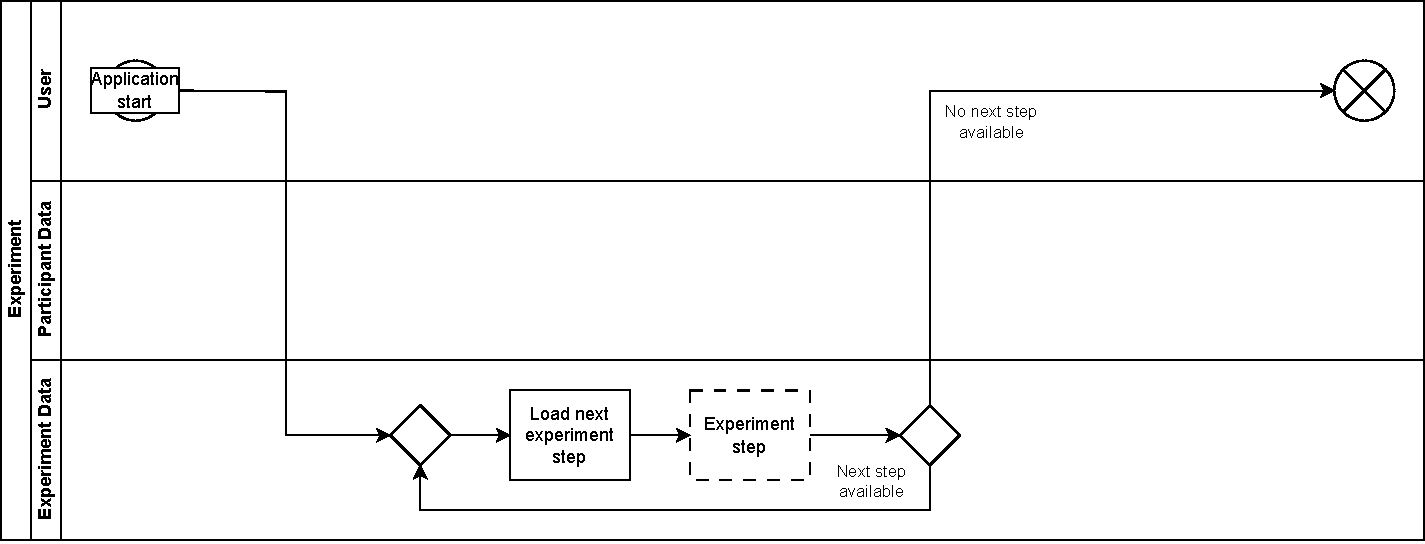
\includegraphics[width=0.99\textwidth, keepaspectratio]{content/05_design_and_dev_artefacts/ExperimentSwimLane.drawio.pdf}
    \caption{Experiment - Swim lane}    
    \label{fig:experimentSwimLane}
\end{figure}

\begin{figure}[htbp]
    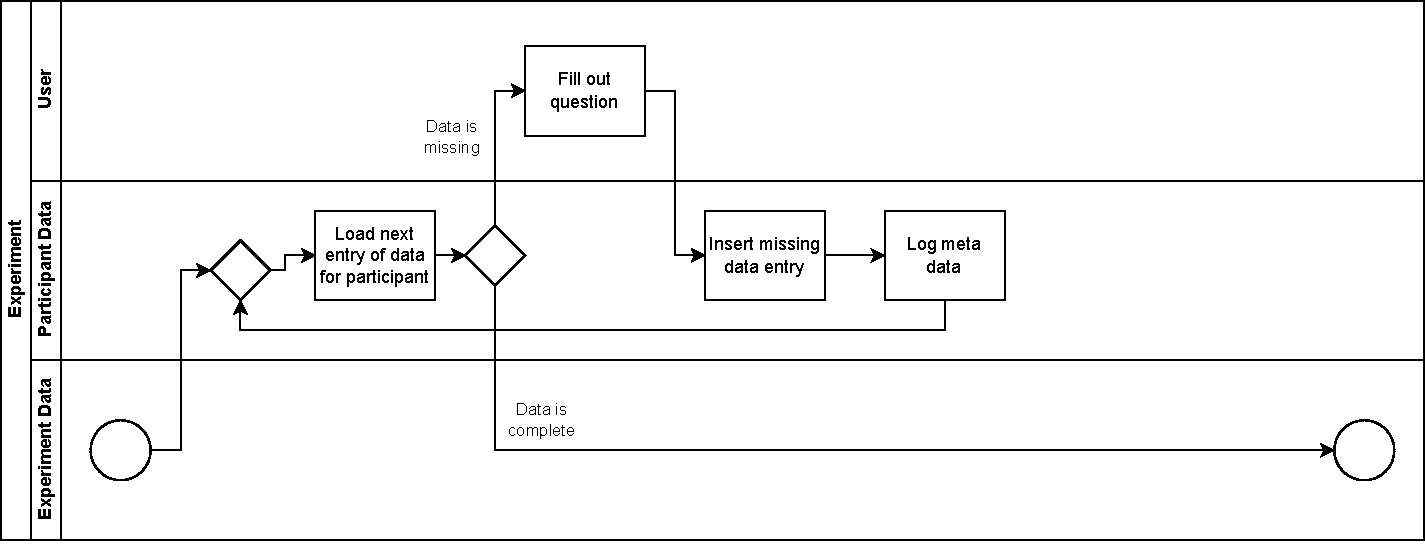
\includegraphics[width=0.99\textwidth, keepaspectratio]{content/05_design_and_dev_artefacts/QuestionairSwimLane.drawio.pdf}
    \caption{Questionair step - Swim lane}    
    \label{fig:questionairSwimLane}
\end{figure}

\begin{figure}[htbp]
    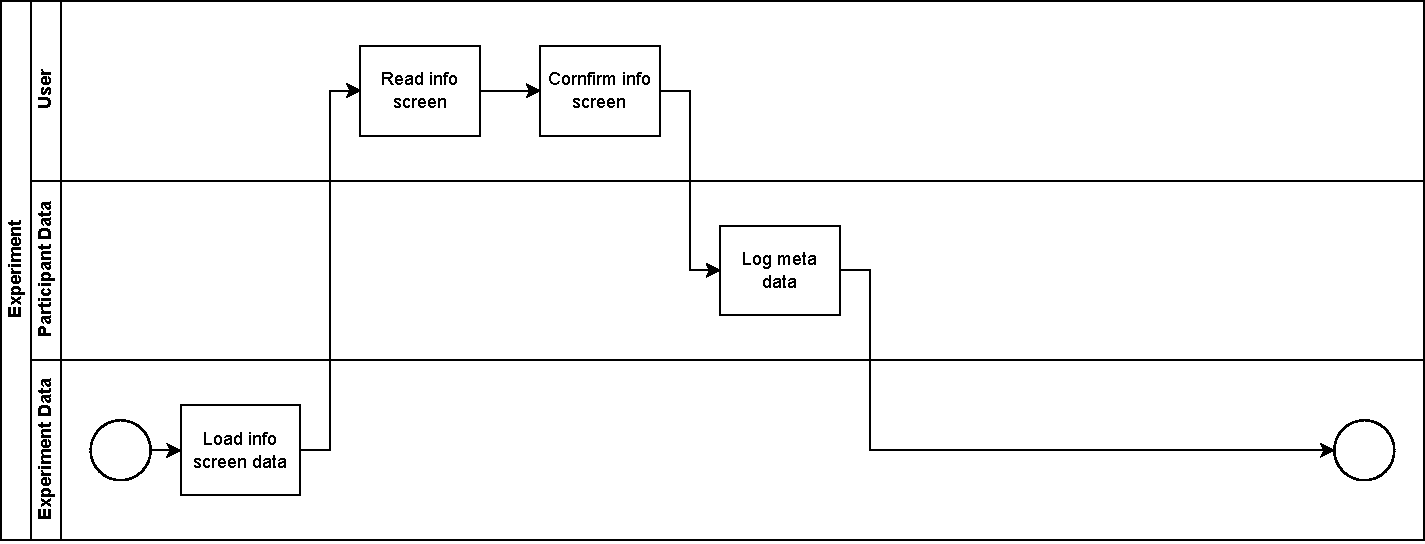
\includegraphics[width=0.99\textwidth, keepaspectratio]{content/05_design_and_dev_artefacts/InfoScreenSwimLane.drawio.pdf}
    \caption{Info screen step - Swim lane}    
    \label{fig:infoScreenSwimLane}
\end{figure}


Customizing ist blöd (\cite{Chou.2008})

\subsubsection{Customizing and System Output}

\subsubsection{Activitys}

%\subsection{Prototype Development}
